\documentclass{article}

\usepackage{amsmath}
\usepackage{amssymb}
\usepackage{hyperref}
\usepackage{indentfirst}
\usepackage{matlab-prettifier}
\usepackage[shortlabels]{enumitem}
\usepackage{graphicx}

%User defined commands
\newcommand{\inv}[1]{#1^{-1}}
\newcommand{\abs}[1]{|#1|}
\newcommand{\norm}[1]{||#1||}
\newcommand{\cond}{\kappa_{||\cdot||}}

\begin{document}
\begin{center}
	\huge{\bf Math 170A: Homework 3} \\
	Merrick Qiu
\end{center}

\section*{Question 1}
    \[
        ||A|| = ||\alpha I|| = |\alpha| ||I|| = |\alpha|
    \]
    \[
        ||A^{-1}|| = ||\frac{1}{\alpha} I||= |\frac{1}{\alpha}|||I|| = |\frac{1}{\alpha}|
    \]
    \[
        \det(A) = \det(\alpha I) = \alpha^n\det(I) = \alpha^n
    \]
    \[
        \cond(A) = \norm{A}\norm{\inv{A}} = \alpha \cdot \frac{1}{\alpha} = 1
    \]

\section*{Question 2}
\begin{enumerate}[(a)]
    \item \begin{align*}
        \kappa(A) &= \norm{A} \cdot \norm{\inv{A}}\\ 
        &= \norm{\inv{A}} \cdot \norm{A} \\
        &= \kappa(\inv{A})
    \end{align*}
    \item From class we know that for $Ax = b$
    \[  
        \frac{\norm{\delta x}}{\norm{x}} \leq \kappa(A) \cdot \frac{\norm{\delta b}}{\norm{b}}
    \]
    Substituting in $A \rightarrow \inv{A}$, $x \rightarrow b$, and $b \rightarrow x$
    and using the equality from part (a) yields
    \begin{align*}
        \frac{\norm{\delta b}}{\norm{b}} &\leq \kappa(\inv{A}) \cdot \frac{\norm{\delta x}}{\norm{x}} \\
        \implies \frac{\norm{\delta b}}{\norm{b}} &\leq \kappa(A) \cdot \frac{\norm{\delta x}}{\norm{x}}
    \end{align*}
\end{enumerate}

\section*{Question 3}
\begin{enumerate}[(a)]
    \item \[
        \norm{A}_1 = \max_{j} \sum_i \abs{a_{ij}} = \max \{5, 1, 5\} = 5
    \]
    \[
        \norm{A}_\infty = \max_{i} \sum_j \abs{a_{ij}} = \max \{5, 4, 2\} = 5
    \]
    \[
        \norm{A}_F =  \sqrt{3^2 + 3\cdot2^2 + 2\cdot 1^2} = \sqrt{23}
    \]
    \item The inverse of A is 
    \[  
        \inv{A} = \frac{1}{10} 
        \begin{bmatrix}
            2 & 2 & 0 \\
            -2 & 3 & 10 \\
            2 & -3 & 0
        \end{bmatrix}
    \]
    Its norms are
    \[
        \norm{\inv{A}}_1 = \max_{j} \sum_i \abs{a_{ij}} = \frac{1}{10}\max \{6, 8, 10\} = 1
    \]
    \[
        \norm{\inv{A}}_\infty = \max_{i} \sum_j \abs{a_{ij}} = \frac{1}{10}\max \{4, 15, 5\} = \frac{3}{2}
    \]
    \[
        \norm{\inv{A}}_F =  \frac{1}{10}\sqrt{10^2 + 2\cdot3^2 + 4\cdot 2^2} = \sqrt{1.34}
    \]
    The condition numbers are 
    \[
        \kappa_1(A) = 5\cdot 1 = 5
    \]
    \[
        \kappa_\infty(A) = 5\cdot\frac{3}{2} = \frac{15}{2}
    \]
    \[
        \kappa_F(A) = \sqrt{23}\cdot \sqrt{1.34} \approx 5.5516
    \]
    \item Dividing the companion inequality by $\kappa(A)$ yields 
    \[
        \frac{\norm{\delta b}}{\kappa(A)\norm{b}} \leq \frac{\norm{\delta x}}{\norm{x}}
    \]
    Under all the norms, $\delta b$ has norm $\epsilon$, so the relative error can be bounded by 
    \[
        \frac{\epsilon}{\kappa(A)\norm{b}} \leq \frac{\norm{\delta x}}{\norm{x}} \leq \kappa(A) \cdot \frac{\epsilon}{\norm{b}}
    \]
    We can get the specific bounds by substituting in the condition numbers we got from (b).
\end{enumerate}

\section*{Question 4}
    The reasoning is incorrect because it confuses the vector itself with its norm.
    Although it might be true that $0.01x = \inv{A}(0.01b)$,
    by submultiplicativity we have that $0.01\norm{x} \leq 0.01\norm{\inv{A}}\norm{b}$
    so a 1 percent change in $b$ can cause a greater than 1 percent change in x 
    if $\norm{\inv{A}}$ is large enough.

\section*{Question 5}
\lstinputlisting[
frame=single,
numbers=left,
style=Matlab-editor
]{question5.m}
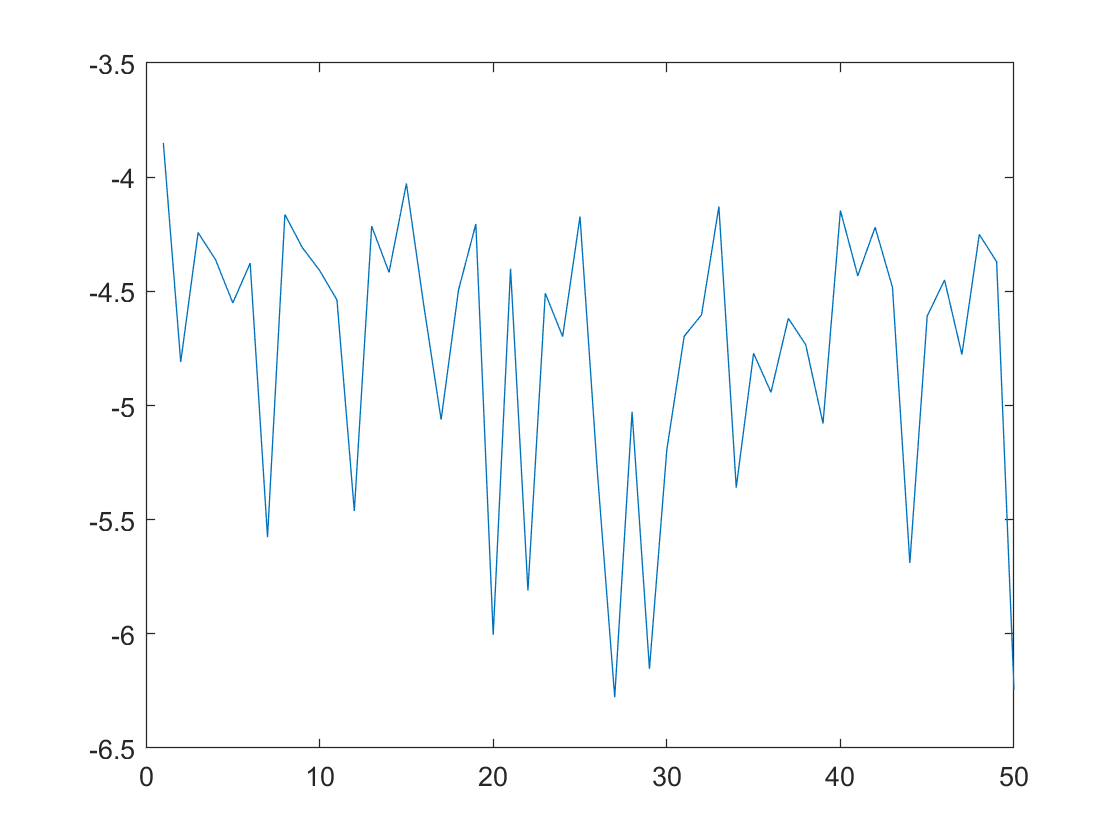
\includegraphics[width = 12cm]{qPlot.png}
Since $\log(q) < 0$ for all the points,
we know that $q < 1$ for all the points,
which agrees with the theory we learned in class.


\end{document}